%--- 31 -------------------------------%
\item\vf{En utilisant une réplication master-slave, une lecture sur le master assurera toujours d’obtenir
les données les plus récentes}
{\vrai}
{Puisque le master est \textbf{le seul noeud accessible en écriture}, ses données sont les plus à jour (contrairement aux esclaves qui doivent être synchronisés).}


%--- 32 -------------------------------%
\item\vf{Les buckets de Riak permettent de segmenter les données en plusieurs collections d’agrégats.}
{}
{Riak est un \textbf{moteur NoSQL décentralisé/distribué} ( = Système de gestion de base de données SGBD) orienté clé-valeur. Il est très bon pour monter en charge, càd augmenter le volume de stockage, et a une haute tolérance aux pannex (peut enlever facilement un noeud en panne sans perte d'intégrité des données).
\paragraph{}
Ce SGBD stocke les clés dans des \textit{\textbf{buckets}}, qui agissent comme des \textbf{espaces de noms} pour les clés. Autrement dit deux clés peuvent porter le même noms si elles se trouvent dans des buckets différents.
\paragraph{}
Dans le modèle clé-valeur, lorsqu'on fait une requête sur une clé, toute la valeur est retournée et il n'est pas possible de cibler certaines parties (gauche fig\cite{fig-riak}). Le système de buckets remédie d'une certaine façon à ce problème en permettant la \textbf{segmentation des données} au sein d'un même bucket (droite fig\cite{fig-riak}). 


\begin{figure}[h!]
\center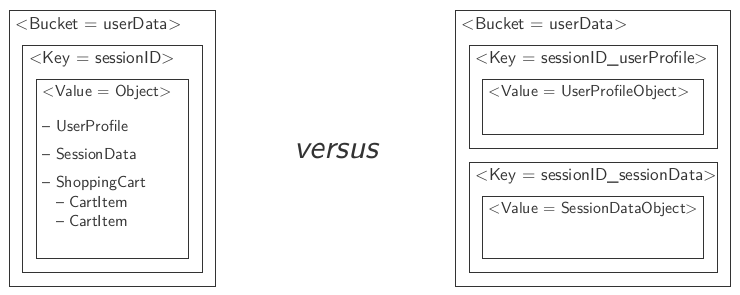
\includegraphics[scale=.3]{images/riak-bucket}
\label{fig-riak}
\caption{Riak - système de \textit{buckets} \cite{ref1}}
\end{figure}

\paragraph{Avantages:}
\begin{itemize}
\item[$\cdot$]pratique lorsqu'on sait que les données d'une même valeur ne seront jamais utilisées en même temps -> évite de récupérer l'ensemble du contenu de la valeur
\end{itemize}
}


%--- 33 -------------------------------%
\item\vf{On ne peut pas stocker des arbres binaires comme valeurs avec Redis.}
{}
{}


%--- 34 -------------------------------%
\item\vf{Redis garantit la persistance de données.}
{}
{}


%--- 35 -------------------------------%
\item\vf{Les bases de données orientée colonnes optimisent le stockage disque pour des tables qui
contiennent de nombreuses lignes.}
{}
{}


%--- 36 -------------------------------%
\item\vf{Une base de données orientée colonnes est très adaptée lorsqu’on a plus d’opérations d’écriture
que de lecture.}
{}
{}

 
%--- 37 -------------------------------%
\item\vf{Une base de données orientée colonnes est très adaptée lorsqu’on a plus d’opérations de lecture
que d’écriture.}
{}
{}


%--- 38 -------------------------------%
\item\vf{Une base de données orientée colonnes est un map à deux niveaux.}
{}
{}


%--- 39 -------------------------------%
\item\vf{Dans une base de données orientée colonnes, les familles de colonnes sont de préférence définies
une fois pour toute lors de la création de la table.}
{}
{}


%--- 40 -------------------------------%
\item\vf{L’avantage de l’utilisation de colonnes plutôt que de lignes est d’offrir une vitesse d’écriture plus grande de nouveaux enregistrements.}
{}
{}
